\section{Nombre: Tlazoltéotl}  \label{per:tlazolteotl}
\subsection{Descripción: }  
De estatura pequeña y gran belleza. De todas las guardianas del Mictlán Tlazoltéotl es quien posee mayor feminidad. Es de piel morena, cabello negro y largo a la altura de la cintura que acostumbra a llevar suelto. De pechos grandes y cadera ancha. Al igual que la mayoria de los Dioses usa joyería de oro fino. En la mano derecha porta una delicada pulsera y en la mano izquierda usa un brazalete con labrados que le cubre casi todo el antebrazo. Usa un par de aretes de jade y un collar de oro adornado con un cuerno de jade de gran tamaño. Tlazoltéotl acostumbra a ir descalza ya que sus movimientos son parecidos a los de una danza y de esta manera se siente mas ligera. Viste un delgado top y una falda que le tiene una ligera abertura entre las piernas, la cual le permite moverse con mayor facilidad.
\\
\par
Tlazoltéotl es de actitud risueña y juguetona pero seductora. Es consciente de la gran belleza que posee y le divierte usarla para confundir a los demás sobre sus intensiones. Disfruta de hablar a manera de acertijo. Posee una mente abierta y dificilmente se sorprende, acostumbra a aburrirse de las cosas rapidamente por lo que le cuetas trabajo enfocarse en sus tareas; sin embargo, desempeña sus deberes con eficiencia una vez que se enfoca.    
\subsection{Status:}
	\begin{itemize}
		\item Personaje no jugable.
		\item Enemigo jefe.
	\end{itemize}
\subsection{Imagen}
Ver figura \ref{fig:TlazolteotlDiseno}
	\begin{figure}
					\centering
					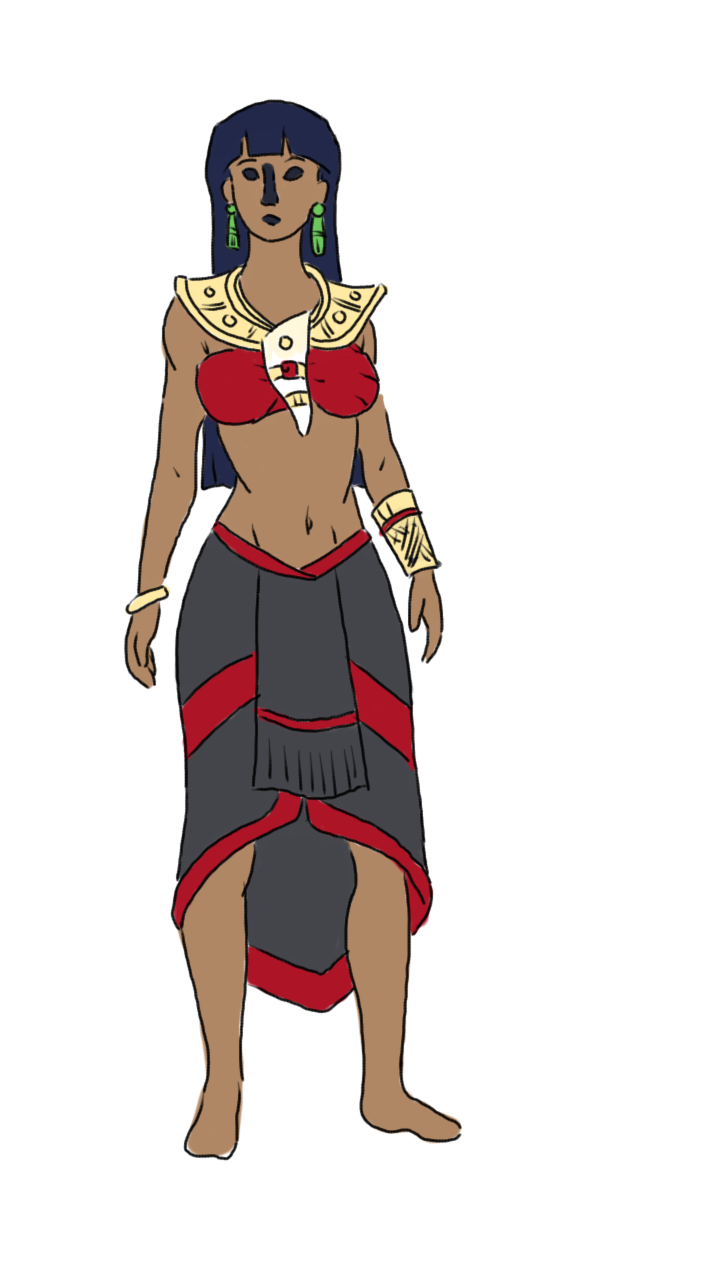
\includegraphics[height=0.3 \textheight]{Imagenes/diosaLujuria}
					\caption{Concepto de diseño de Tlazoltéotl.}
					\label{fig:TlazolteotlDiseno}
	\end{figure}
\subsection{Concepto:}
\begin{itemize}
	\item \textbf{Historia antes del juego:}
	Luego de que uno de los antiguos guardianes del Mictlan cayera en combate durante la guerra contra los dioses del norte, Tezcatlipoca pide volutarios para tomar el puesto. Siendo Tlazoltéotl la unica en ofrecerse para tal tarea. Tlazoltéotl Elige ser guardiana del Mictlán por que tenía curiosidad sobre como eran las almas de los humanos, ya que ella considera que la verdadera cara de las personas se mostraba en la muerte.
	\\
	\par
	El papel de Tlazoltéotl en el Mictlan, ademas de proteger su nivel correspondiente, es el de purificar las almas de las personas cuyas faltas hayan sido de carácter sexual, tal como la infidelidad. A su vez, ella se encarga de darle paz a aquellas almas que hayan muerto durante agresiones de carácter sexual. 
	\item \textbf{Historia durante el juego:}
	El papel de  Tlazoltéotl en el juego se limita a ser un jefe para un nivel en especifico. Es importante remarcar que para  Tlazoltéotl, los invasores solo eran un pequeño inconveniente en un día de trabajo común.
	\item \textbf{Relaciones:}
	\begin{itemize}
		\item \textbf{Xólotl:} Considerado por Tlazoltéotl como un ser debil por el que siente un poco de pena. Encuentra un poco deprimente el hecho de que Xólotl se esfuerce demasiado por ganar la aceptación de los demás (ver aparatado \ref{per:xolotl}). 
		\item \textbf{Malinalli:} Presenta un dilema para la diosa, ya que al ser su enemiga debe de derrotarla pero al observar con sus poderes los horrores a los que ha sido sometida como esclava  Tlazoltéotl desea que Malinalli encuentre pas en su corazón (ver aparatado \ref{per:malinalli}).
	\end{itemize}                     
\end{itemize}

\subsection{Encuentro:}
\begin{itemize}
	\item Su primera aparición es en la cinemática 9 (ver aparatado \ref{Cin:Cinematica09}).
	\item Como jefe, el juagdor se enfrenta a ella en el nivel el sexto nivel del juego (ver aparatado \ref{Nivel:Niv06}).
\end{itemize} 

\subsection{Habilidades:}
\begin{itemize} 
	\item Raíz del diablo (ver aparatado \ref{hab.RaizDia}).
	\item Energía corrupta (ver aparatado \ref{hab.CorrupEner}).
	\item Circulo protector (ver aparatado \ref{hab.CirPro}).
\end{itemize} 
\subsection{Armas:}
Sin armas.
\subsection{Ítems:}
Sin ítems.
\subsection{Bloques de animación}
	\begin{itemize}
		\item Animación vuelo.
		\item Animación disparar energía corrupta.
		\item Animación invocar círculo protector.
		\item Animación disparar raíz diablo.
		\item Animación recibir daño.
		\item Animación morir.
	\end{itemize}